\section{Overview}\seclabel{Overview}

In this section, we informally describe our approach with a few simple example programs.

\subsection{Motivating Example}

\begin{figure}
\centering
\begin{tabular}{ccc}
\begin{lstlisting}
int sign(int x) { 
  int sgn;
  if (x < 0)
    sgn = -1
  else 
    sgn = 1
 return sgn
}
(*@ \vspace{0.1in} @*)
\end{lstlisting}
&
&
\begin{lstlisting}
int sign'(int x) {
  int sgn;
  if (x < 0)
    sgn = -1
  else if (x==0)
    sgn = 0
  else 
    sgn = 1
 return sgn
}
\end{lstlisting}
\\
\end{tabular}
\caption{Two simple implementations of the \emph{sign} operation.}
\figlabel{SignExample}
\end{figure}


Consider the simple example program of~\figref{SignExample}, inspired by an example from~\cite{RM:TOPLAS07}. For this example, we would like to establish that at the exit point of the program, $sign$ and $sign'$ only differ in the case where $x=0$ and that the difference is $sgn = 1 \neq sgn' = 0$.

As a first naive attempt one could try to analyze each version of the program separately and compare the (abstract) results. However, this is clearly unsound, as equivalence under abstraction does not entail concrete equivalence. For example, using a interval analysis~\cite{TODO} would yield that in both programs the value of \scode{sgn} ranges in the same interval $[-1,1]$, missing the fact that $sign$ never returns the value $0$. Furthermore, this result entirely ignores how $x$ affects the value of $sgn$ as the analysis domain is path insensitive.

\paragraph{Establishing equivalence under abstraction}
To establish equivalence under abstraction, we need to abstract relationships between the values of variables in $sign$ and $sign'$ under the assumption of equivalence of input. Specifically, we need to track the relationship between the values of \scode{sgn} in both versions, while assuming $x=x'$, and see whether we can establish their equivalence.

%Question 1: How would be go about performing a joint analysis on 2 separate programs? how would that work?

We reduce the problem of analysis across two programs to the problem of analyzing a single program by constructing a \emph{correlating program}. The correlating program represents the behaviors of both programs, and allows us to reason about relationships between variables in both. 

\begin{figure}
\centering
\begin{lstlisting}
// Nimrod - please fill this 
\end{lstlisting}
\caption{Correlating program $sign \correlate sign'$.}
\figlabel{SignCorrelating}
\end{figure}


\figref{SignCorrelating} shows the correlating program for the programs of ~\figref{SignExample}. The programs were transformed to a guarded command language form to allow for interleaving. Using the correlating program, we can directly track the relationship between \scode{sgn} in $sign$ and its corresponding variable \scode{sgn'} in $sign'$. Unfortunately, any domain with convex constraints will still fail to capture the precise relationship between \scode{sgn} and \scode{sgn'}. For example, using the polyhedra abstract domain~\cite{TODO}, the relationship between \scode{sgn} and \scode{sgn'} in the correlating program would be lost, leaving only the trivial $\langle 1 \geq sgn \geq -1, 1 \geq sgn' \geq -1 \rangle$ constraint. Although the result soundly reports a difference, we still know nothing of the difference between the programs.

An obvious, but prohibitively expensive, solution to the problem is to use disjunctive completion~\cite{TODO}, moving to a powerset domain in which every abstract state is a set of convex objects (e.g., set of polyhedra). However, using such domain would significantly limit the applicability of the approach.

The desirable solution is a partially disjunctive domain, in which only certain disjunctions are kept separate during the analysis, while others are merged. The challenge in our setting is in keeping the partition fine enough such that equivalence could be preserved, without reaching exponential blowup.

\paragraph{How to partition}
We base our choice of explicit disjunctions to be kept based on their effect on variable equivalence. We partition the disjunctions according to equivalence criteria, specifically the set of variables for which equivalence is held for. This equivalence-oriented partition is natural, considering our problem domain. Using this partially disjunctive domain on \figref{SignCorrelating} will produce a much precise result containing the disjunction $\langle \neg g2, \equiv_{sgn,x,g1} \rangle \vee \langle g1, \equiv_{x,g1}, x' = 0, sgn' = 0 \rangle$. The domain's equivalence preserving properties allow for a temporary divergence of equality as a step of $sign$ was interpreted, only to restore equivalence once the corresponding step from $sign'$ was considered. This expresses the correlating program's part in allowing for such analysis by supplying the appropriate interleaving.

To further establish the importance of the correlating program, let us consider previous approaches ~\cite{}, which suggest performing an analysis of the sequential composition of the programs. \figref{SignSequential} shown a sequential composition of the $sign$ and $sign'$ programs. Achieving a similar result using the sequential program requires using the disjunctive completion domain where no partitioning can be performed. \figref{SignSequentialAnalysis} shows the analysis process for $sign';sign$ control flow graph. Applying a merge at any of the merge points will result in a permanent lose of equivalence. Essentially, in the sequential program, the analysis must "wait" the length of the entire procedure until it reaches the appropriate location in second procedure which will allow it to assume equivalence. Our correlating program circumvents this need.

\begin{figure}
\centering
\begin{lstlisting}
int sign_sign'(int x) {
  int sgn' = sign'(x);
  int sgn = sign(x);
  assert(sgn == sgn');
}
\end{lstlisting}
\caption{Sequential composition of programs $sign ; sign'$.}
\figlabel{SignCorrelating}
\end{figure}

\begin{figure}
\imagetop{
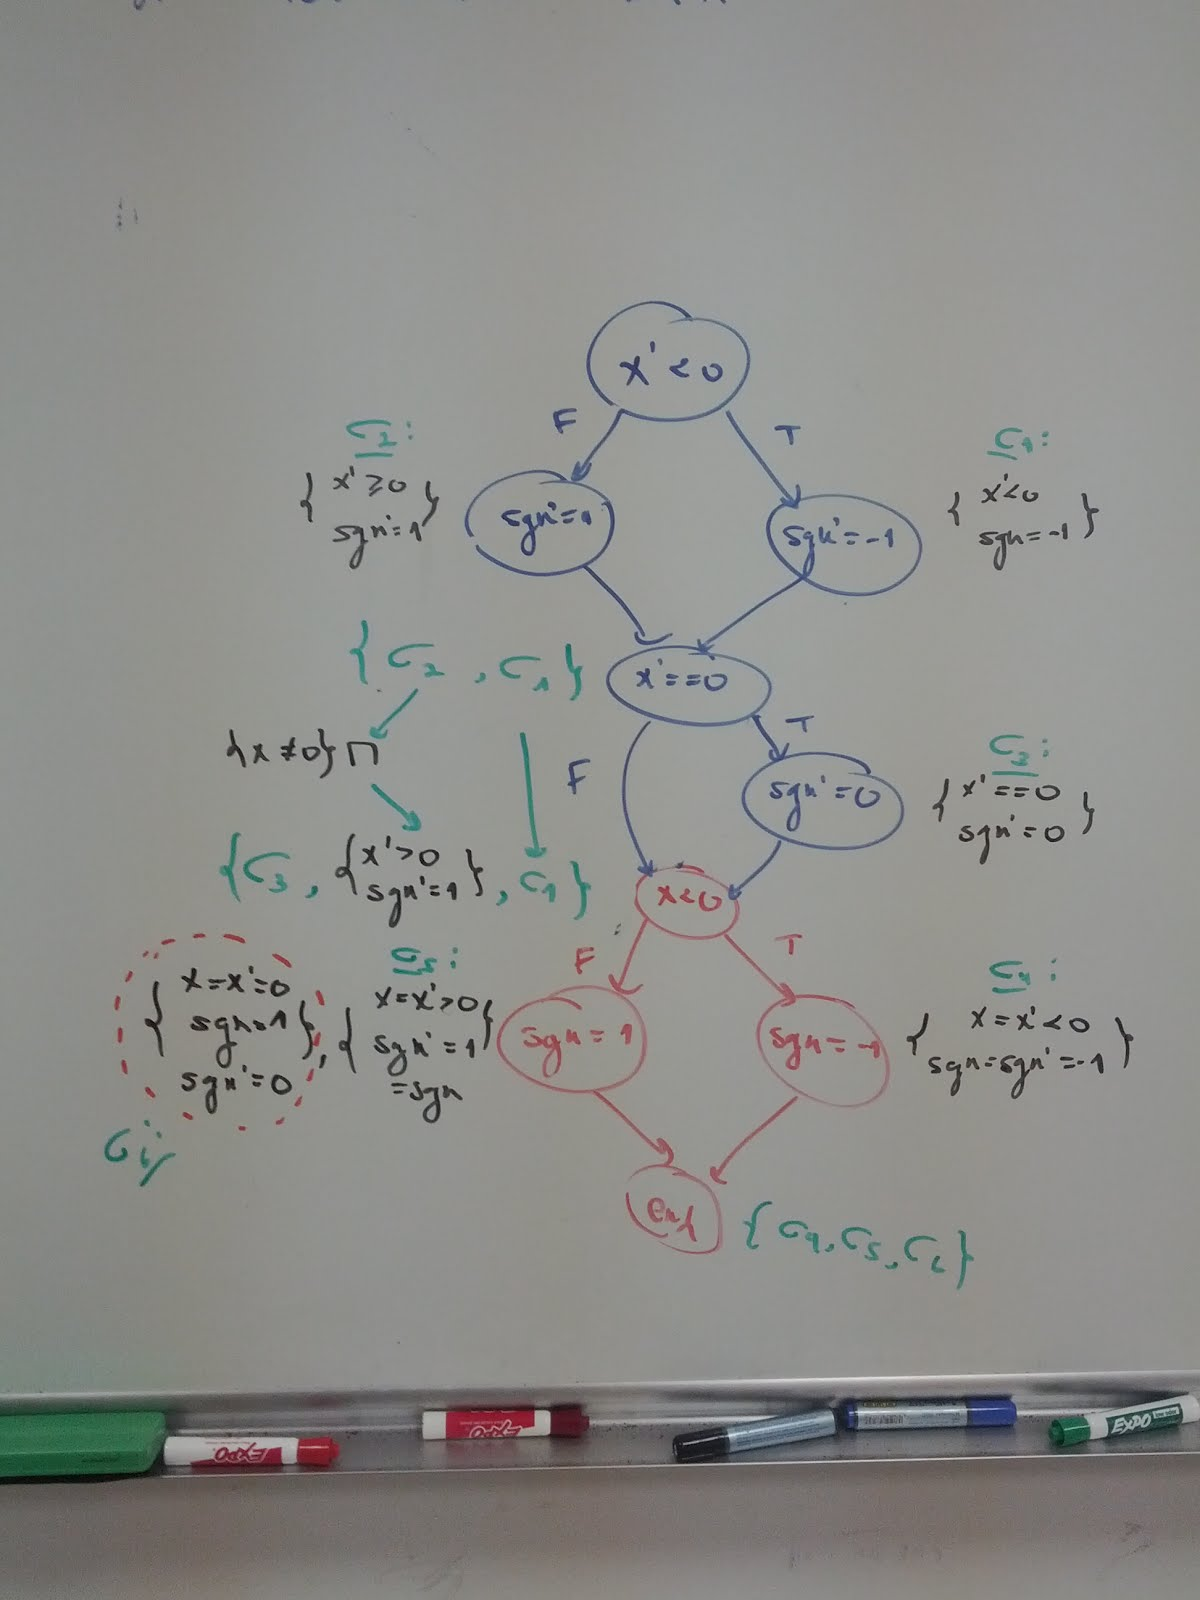
\includegraphics[scale=0.22,clip=true,trim = 75pt 300pt 50pt 250pt]{figures/sign-seq-analysis.jpg}
}
\caption{Sequential $sign';sign$ analysis}\figlabel{SignSequentialAnalysis}
\end{figure}

\ignore{
An alternative way to track the state across both programs is to define a correlating semantics (e.g., \cite{TODO}) where both programs are executed in lock-step and then abstract this correlating semantics.
}

\paragraph{Widening}

